\documentclass[12pt,a4paper]{article}

% --- Page Layout -------------------------------------------------------------
\usepackage[a4paper, top=0.8in, bottom=1.1in, left=0.8in, right=0.8in, headheight=14pt, footskip=30pt]{geometry}

% --- Fonts (XeLaTeX) ---------------------------------------------------------
\usepackage{fontspec}
\usepackage{unicode-math}
\setmainfont{TeX Gyre Pagella}
\setmonofont[Scale=0.88]{TeX Gyre Cursor}
\setmathfont{Latin Modern Math}

% --- Packages ---------------------------------------------------------------
\usepackage{xcolor}
\usepackage{titlesec}
\usepackage{enumitem}
\usepackage{tabularx}
\usepackage{booktabs}
\usepackage{array}
\usepackage{amsmath}
\usepackage{tikz}
\usetikzlibrary{shapes.geometric, arrows.meta, positioning, calc, fit,
                decorations.pathreplacing, decorations.pathmorphing}
\usepackage{tcolorbox}
\tcbuselibrary{skins, breakable}
\usepackage{hyperref}
\usepackage{fancyhdr}
\usepackage{graphicx}
\usepackage{microtype}
\hyphenpenalty=10000
\exhyphenpenalty=10000
\sloppy
\usepackage{caption}
\usepackage{setspace}
\usepackage{multirow}
\usepackage{tocloft}

% --- Q&A helper --------------------------------------------------------------
\newcommand{\Q}[1]{\textbf{#1}\par\noindent\ignorespaces}

% --- Colour Palette ----------------------------------------------------------
\definecolor{myred}{RGB}{196,30,58}
\definecolor{mydark}{RGB}{30,30,50}
\definecolor{mygreen}{RGB}{14,120,80}
\definecolor{myteal}{RGB}{0,130,140}
\definecolor{myamber}{RGB}{180,100,0}
\definecolor{mypurple}{RGB}{100,30,160}
\definecolor{mygray}{RGB}{246,247,249}
\definecolor{mgframe}{RGB}{180,185,200}
\definecolor{watermark}{RGB}{145,150,170}
\definecolor{hdrred}{RGB}{250,232,235}
\definecolor{hdrgreen}{RGB}{220,244,233}
\definecolor{hdrteal}{RGB}{220,242,244}
\definecolor{hdramber}{RGB}{253,242,215}
\definecolor{hdrpurple}{RGB}{238,228,255}
\definecolor{hdrgray}{RGB}{238,240,245}
\definecolor{rowalt}{RGB}{250,251,253}

% --- Section Formatting ------------------------------------------------------
\titleformat{\section}
  {\large\bfseries\color{myred}}{\thesection.}{0.5em}{}
  [\vspace{1pt}{\color{myred}\rule{\linewidth}{0.8pt}}]
\titleformat{\subsection}
  {\normalsize\bfseries\color{myteal}}{\thesubsection}{0.5em}{}
\titlespacing*{\section}{0pt}{18pt}{7pt}
\titlespacing*{\subsection}{0pt}{11pt}{4pt}

% --- Paragraph ---------------------------------------------------------------
\setlength{\parindent}{0pt}
\setlength{\parskip}{4pt}

% --- Page filling ------------------------------------------------------------
\raggedbottom

% --- TOC Styling -------------------------------------------------------------
\renewcommand{\cfttoctitlefont}{\large\bfseries\color{myred}}
\renewcommand{\cftaftertoctitle}{\par\noindent{\color{myred}\rule{\linewidth}{0.8pt}}}
\setlength{\cftbeforetoctitleskip}{0pt}
\setlength{\cftaftertoctitleskip}{6pt}
\renewcommand{\cftsecfont}{\normalsize\bfseries\color{mydark}}
\renewcommand{\cftsecpagefont}{\normalsize\bfseries\color{mydark}}
\renewcommand{\cftsecleader}{\cftdotfill{\cftdotsep}}
\setlength{\cftbeforesecskip}{7pt}
\renewcommand{\cftsubsecfont}{\small\color{mydark}}
\renewcommand{\cftsubsecpagefont}{\small\color{mydark}}
\setlength{\cftbeforesubsecskip}{3pt}
\setlength{\cftsubsecindent}{1.4em}

% --- Table helpers -----------------------------------------------------------
\renewcommand{\arraystretch}{1.45}
\setlength{\tabcolsep}{6pt}
\newcolumntype{B}[1]{>{\small\bfseries\raggedright\arraybackslash}m{#1}}
\newcolumntype{Y}{>{\small\raggedright\arraybackslash}X}
\renewcommand{\tabularxcolumn}[1]{m{#1}}

% --- Header / Footer ---------------------------------------------------------
\pagestyle{fancy}
\fancyhf{}
\fancyhead[L]{\small\color{myred}\textbf{BS-CH101}\;\color{mydark}--- Chemistry-I}
\fancyhead[R]{\small\color{myteal}\textbf{Module 3 Long Notes}}
\fancyfoot[L]{\small\color{watermark}\textit{\copyright\ MAKAUT Wingman}}
\fancyfoot[C]{\small\color{mydark}\thepage}
\fancyfoot[R]{\small\color{watermark}\textit{\copyright\ Biraj}}
\renewcommand{\headrulewidth}{0.5pt}
\renewcommand{\footrulewidth}{0.3pt}

% --- Hyperref ---------------------------------------------------------------
\hypersetup{
  colorlinks=true, linkcolor=myteal, urlcolor=myteal,
  pdfauthor={Biraj Sarkar},
  pdftitle={BS-CH101 --- Module 3 Long Notes: Intermolecular Forces and Real Gases}
}

% --- tcolorbox styles --------------------------------------------------------
\tcbset{
  tikzbox/.style={
    colback=mygray, colframe=mgframe, boxrule=0.6pt, arc=4pt,
    left=8pt, right=8pt, top=6pt, bottom=6pt,
    colbacktitle=mgframe, coltitle=mydark, fonttitle=\small\bfseries
  },
  defbox/.style={
    colback=hdrgreen, colframe=mygreen, boxrule=0.8pt, arc=4pt,
    left=9pt, right=9pt, top=6pt, bottom=6pt,
    colbacktitle=mygreen, coltitle=white, fonttitle=\small\bfseries
  },
  formulabox/.style={
    colback=hdrteal, colframe=myteal, boxrule=0.8pt, arc=4pt,
    left=9pt, right=9pt, top=7pt, bottom=7pt,
    colbacktitle=myteal, coltitle=white, fonttitle=\small\bfseries
  },
  examplebox/.style={
    colback=hdramber, colframe=myamber, boxrule=0.8pt, arc=4pt,
    left=9pt, right=9pt, top=6pt, bottom=6pt,
    colbacktitle=myamber, coltitle=white, fonttitle=\small\bfseries
  },
  masonbox/.style={
    colback=hdrpurple, colframe=mypurple, boxrule=0.8pt, arc=4pt,
    left=9pt, right=9pt, top=6pt, bottom=6pt,
    colbacktitle=mypurple, coltitle=white, fonttitle=\small\bfseries
  },
  exambox/.style={
    colback=hdrpurple, colframe=mypurple, boxrule=1pt, arc=5pt,
    left=10pt, right=10pt, top=8pt, bottom=8pt,
    colbacktitle=mypurple, coltitle=white, fonttitle=\bfseries,
    breakable, title after break={\textbf{Frequently Asked / Viva Questions (contd.)}}}
}
\tcbset{breakable}

% --- TikZ styles -------------------------------------------------------------
\tikzset{
  block/.style={rectangle, draw=myteal, fill=hdrteal,
    text width=2.4cm, align=center, minimum height=0.95cm,
    font=\small, rounded corners=3pt, line width=0.7pt},
  redblock/.style={rectangle, draw=myred, fill=hdrred,
    text width=2.4cm, align=center, minimum height=0.95cm,
    font=\small, rounded corners=3pt, line width=0.7pt},
  netnode/.style={rectangle, draw=myteal, fill=hdrteal,
    text width=1.5cm, align=center, minimum height=0.8cm,
    font=\small, rounded corners=3pt, line width=0.7pt},
  sumjunc/.style={circle, draw=myamber, fill=hdramber,
    minimum size=0.62cm, font=\small, line width=0.8pt},
  snode/.style={circle, draw=mypurple, fill=hdrpurple,
    minimum size=0.55cm, font=\footnotesize, line width=0.7pt},
  arrow/.style={-Stealth, thick, color=mydark},
  redarrow/.style={-Stealth, thick, color=myred},
  line/.style={thick, color=mydark}
}

\begin{document}

\begin{center}
  {\LARGE\bfseries\color{myred} BS-CH101 / BS-CH201 --- Chemistry-I}\\[5pt]
  {\normalsize\color{mydark} Semester I/II \quad$\bullet$\quad 3L:1T:0P \quad$\bullet$\quad 4 Credits}\\[3pt]
  {\normalsize\color{myteal}\textbf{Module 3 Long Notes: Intermolecular Forces, Real Gases and Critical Phenomena}}\\[3pt]
  {\small\color{mydark} CGEC \;$|$\; B.Tech ECE (2023--27) \;$|$\; \textit{Biraj Sarkar}}
\end{center}
\vspace{2pt}
\noindent{\color{myred}\rule{\linewidth}{1.5pt}}
\vspace{2pt}
\hypersetup{linkcolor=mydark}
\tableofcontents
\hypersetup{linkcolor=myteal}
\newpage
% ===============================================================================
\section{Intermolecular Forces: Classification and Origin}
% ===============================================================================

\begin{tcolorbox}[defbox]
\textbf{Intermolecular forces (IMF)} are attractive or repulsive forces between molecules, atoms, or ions that are not covalently bonded. They arise from electrostatic interactions between charge distributions and are the cause of condensation, surface tension, viscosity, solubility, and deviation from ideal-gas behaviour. They are \emph{weaker} than intramolecular (covalent/ionic) bonds but collectively determine the physical state and material properties of matter.
\end{tcolorbox}

\subsection{Classification of Intermolecular Forces}
All intermolecular forces can be traced to Coulomb's law: $V \propto q_1 q_2 / r$. Depending on whether the charges are permanent, induced, or fluctuating, we get different categories.

\begin{tabularx}{\linewidth}{|B{2.8cm}|Y|Y|Y|}
\hline
\textbf{Force} & \textbf{Between} & \textbf{Origin} & \textbf{Example} \\
\hline
Ion--ion & Two ions & Full charges $q_1q_2$ & NaCl lattice \\
\hline
Ion--dipole & Ion + polar molecule & Charge + permanent dipole & $\mathrm{Na^+}$--water hydration \\
\hline
Dipole--dipole (Keesom) & Two polar molecules & Two permanent dipoles & HCl--HCl, acetone \\
\hline
Dipole--induced dipole (Debye) & Polar + polarisable molecule & Permanent dipole induces temporary dipole & HCl--Ar \\
\hline
Dispersion (London) & Any two molecules & Instantaneous dipole--induced dipole & Ar--Ar, $\mathrm{CH_4}$ \\
\hline
Hydrogen bonding & H covalently bonded to F, O, N & Electrostatic + partial covalent & Water, HF, DNA \\
\hline
\end{tabularx}

\subsection{Ionic Interactions}
An ionic interaction is the electrostatic attraction between oppositely charged ions. It is the strongest non-covalent force.

\begin{tcolorbox}[formulabox, title={Coulomb Potential Between Two Ions}]
\[
V_{\mathrm{ion-ion}}=-\frac{z_1 z_2 e^2}{4\pi\varepsilon_0 r}
\]
$z_1, z_2$ = signed charge numbers; $e=1.602\times10^{-19}\ \mathrm{C}$; $r$ = interionic distance; $\varepsilon_0=8.854\times10^{-12}\ \mathrm{C^2\,N^{-1}\,m^{-2}}$.\\[2pt]
Energy falls as $1/r$ (long range). In a crystal, many-ion Madelung sums give the lattice energy.
\end{tcolorbox}

\textbf{Lattice energy and Born--Haber cycle:} The Born--Haber cycle uses Hess's law to evaluate the lattice energy $U_L$ indirectly, since direct measurement is impossible:
\[
U_L = \Delta H_f^\circ(\mathrm{salt}) - \Delta H_{\mathrm{sub}} - \Delta H_{\mathrm{IE}} - \tfrac12 \Delta H_{\mathrm{diss}} - \Delta H_{\mathrm{EA}}
\]
Higher lattice energy means harder crystal, higher melting point. $\mathrm{MgO}$ ($U_L\approx3850\ \mathrm{kJ\,mol^{-1}}$) is harder than $\mathrm{NaCl}$ ($U_L\approx787\ \mathrm{kJ\,mol^{-1}}$) because $\mathrm{Mg^{2+}/O^{2-}}$ charges are double.

\subsection{Dipole Moment and Polar Molecules}

\begin{tcolorbox}[defbox]
\textbf{Dipole moment} $\vec{\mu}$ arises whenever positive and negative charge centres do not coincide. For a diatomic $\mathrm{A{-}B}$: $\mu = q\cdot d$, where $q$ is the partial charge and $d$ is the bond length. Units: debye (D), $1\ \mathrm{D}=3.336\times10^{-30}\ \mathrm{C\,m}$.
\end{tcolorbox}

\begin{tabularx}{\linewidth}{|B{2.6cm}|Y|Y|}
\hline
\textbf{Molecule} & \textbf{$\mu$ (D)} & \textbf{Comment} \\
\hline
$\mathrm{H_2O}$ & 1.85 & Bent structure, dipoles add \\
\hline
$\mathrm{NH_3}$ & 1.47 & Pyramidal \\
\hline
$\mathrm{HCl}$ & 1.08 & Heteronuclear diatomic \\
\hline
$\mathrm{CO_2}$ & 0 & Linear, dipoles cancel \\
\hline
$\mathrm{CCl_4}$ & 0 & Tetrahedral, dipoles cancel \\
\hline
$\mathrm{CHCl_3}$ & 1.01 & Asymmetric tetrahedral \\
\hline
\end{tabularx}

\textbf{Why $\mathrm{CO_2}$ and $\mathrm{CCl_4}$ are non-polar:} Each individual bond is polar but the vector sum of all bond dipoles is zero due to the symmetric geometry.

\subsection{Dipole--Dipole (Keesom) Interaction}
Two polar molecules attract when oppositely charged ends face each other and repel when like ends face. After thermal averaging over all orientations:

\begin{tcolorbox}[formulabox, title={Keesom Orientational Energy (Thermal Average)}]
\[
V_{\mathrm{Keesom}} = -\frac{2\mu_1^2\mu_2^2}{3(4\pi\varepsilon_0)^2 k_B T\,r^6}
\]
Key feature: falls as $r^{-6}$ and is temperature-dependent (decreases at higher $T$ because thermal motion disrupts orientation).
\end{tcolorbox}

\subsection{Dipole--Induced Dipole (Debye) Interaction}
A polar molecule distorts the electron cloud of a nearby polarisable, non-polar molecule creating an induced dipole. The interaction is always attractive.

\begin{tcolorbox}[formulabox, title={Debye Induction Energy}]
\[
V_{\mathrm{Debye}} = -\frac{\mu^2\alpha'}{(4\pi\varepsilon_0)^2 r^6}
\]
$\alpha'$ = polarisability volume (SI: $\mathrm{C^2\,m^2\,J^{-1}}$; often tabulated in \r{A}$^3$). Like Keesom, falls as $r^{-6}$ but is \emph{temperature-independent}.
\end{tcolorbox}

\subsection{London Dispersion Forces}
Even completely non-polar atoms/molecules (noble gases, hydrocarbons) attract each other and can be liquefied. This requires a quantum-mechanical explanation.

\begin{tcolorbox}[defbox]
\textbf{London dispersion (induced-dipole--induced-dipole) force:} At any instant, the electron distribution in an atom fluctuates, creating a transient dipole. This instantaneous dipole polarises a neighbouring atom, inducing a correlated dipole. The time-averaged interaction is always \emph{attractive}.
\end{tcolorbox}

\begin{tcolorbox}[formulabox, title={London Dispersion Energy}]
\[
V_{\mathrm{London}} = -\frac{3}{2}\,\frac{\alpha_1'\alpha_2'}{(4\pi\varepsilon_0)^2 r^6}\cdot\frac{I_1 I_2}{I_1+I_2}
\]
$I_1, I_2$ = ionisation energies; $\alpha_1', \alpha_2'$ = polarisability volumes.\\
Key: falls as $\boldsymbol{r^{-6}}$; increases with polarisability (larger molecules, more electrons, heavier atoms).
\end{tcolorbox}

\textbf{Why dispersion forces increase down a group:}

\begin{tabularx}{\linewidth}{|B{2.4cm}|Y|Y|Y|}
\hline
\textbf{Noble gas} & \textbf{Polarisability (pm$^3$)} & \textbf{Boiling point (K)} & \textbf{Trend} \\
\hline
He & 2.3 & 4.2 & \\
\hline
Ne & 4.0 & 27.1 & \\
\hline
Ar & 16.3 & 87.3 & Increasing down \\
\hline
Kr & 24.8 & 119.9 & \\
\hline
Xe & 40.4 & 165.1 & \\
\hline
\end{tabularx}

\begin{tcolorbox}[examplebox, title={Solved Example: Why Hexane Boils at 69$^\circ$C but Pentane at 36$^\circ$C}]
Both are non-polar and rely on London dispersion only. Hexane ($\mathrm{C_6H_{14}}$, MW = 86) has more electrons and higher polarisability than pentane ($\mathrm{C_5H_{12}}$, MW = 72). The stronger London forces require more energy to overcome, raising the boiling point by $\sim33^\circ\mathrm{C}$.
\end{tcolorbox}

\subsection{Hydrogen Bonding}
Hydrogen bonding is the strongest intermolecular interaction between neutral molecules ($15$--$40\ \mathrm{kJ\,mol^{-1}}$, about 10--20\% of a covalent bond). It requires:
\begin{enumerate}[leftmargin=*, itemsep=1pt, topsep=2pt]
  \item A hydrogen covalently bonded to a highly electronegative atom (F, O, or N) --- the \emph{donor}.
  \item A nearby lone pair on another electronegative atom --- the \emph{acceptor}.
\end{enumerate}

\begin{tcolorbox}[tikzbox, title={Hydrogen Bonding in Water}]
\centering
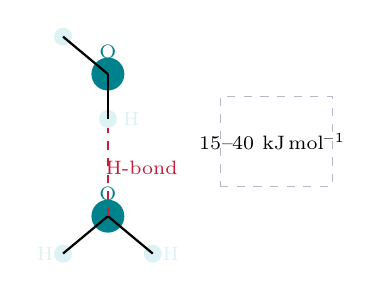
\begin{tikzpicture}[scale=0.95]
  % Molecule 1
  \fill[myteal]   (0,0) circle (0.22) node[above=2pt, font=\scriptsize] {O};
  \fill[hdrteal]  (-0.6,-0.5) circle (0.12) node[left, font=\scriptsize] {H};
  \fill[hdrteal]  (0.6,-0.5) circle (0.12) node[right, font=\scriptsize] {H};
  \draw[thick] (0,0)--(-0.6,-0.5);
  \draw[thick] (0,0)--(0.6,-0.5);
  % H-bond
  \draw[dashed, myred, thick] (0,0)--(0,1.3);
  \node[font=\scriptsize, color=myred] at (0.45,0.65) {H-bond};
  % Molecule 2
  \fill[myteal]   (0,1.9) circle (0.22) node[above=2pt, font=\scriptsize] {O};
  \fill[hdrteal]  (-0.6,2.4) circle (0.12);
  \fill[hdrteal]  (0,1.3)    circle (0.12) node[right=2pt, font=\scriptsize] {H};
  \draw[thick] (0,1.9)--(-0.6,2.4);
  \draw[thick] (0,1.9)--(0,1.3);
  \node[font=\scriptsize] at (2.2,1.0) {$15$--$40\ \mathrm{kJ\,mol^{-1}}$};
  \draw[dashed, mgframe] (1.5,0.4)--(3.0,0.4)--(3.0,1.6)--(1.5,1.6)--cycle;
\end{tikzpicture}
\end{tcolorbox}

\textbf{Consequences of hydrogen bonding:}
\begin{itemize}[leftmargin=*, itemsep=2pt, topsep=2pt]
  \item Anomalously high boiling points: water (100$^\circ$C) vs $\mathrm{H_2S}$ ($-60^\circ$C), HF (19.5$^\circ$C) vs HCl ($-85^\circ$C).
  \item High heat of vaporisation of water ($44\ \mathrm{kJ\,mol^{-1}}$).
  \item Ice is less dense than liquid water (open hydrogen-bonded network).
  \item Protein secondary structure (alpha helix: $i$ to $i+4$ N--H$\cdots$O$=$C).
  \item DNA double helix held by A--T (2 H-bonds) and G--C (3 H-bonds) base pairing.
\end{itemize}

\textbf{Intermolecular vs intramolecular H-bonding:}\par\noindent
\begin{tabularx}{\linewidth}{|B{3.2cm}|Y|Y|}
\hline
\textbf{Type} & \textbf{Occurs between} & \textbf{Effect} \\
\hline
Intermolecular & Different molecules & Higher bp, greater association in solution \\
\hline
Intramolecular & Within same molecule & Lower bp than without H-bond; less association \\
\hline
\end{tabularx}

Example: \emph{ortho}-nitrophenol has an intramolecular H-bond between OH and the adjacent $\mathrm{NO_2}$; \emph{para}-nitrophenol cannot, so it forms intermolecular H-bonds and has a higher melting point.

\subsection{Polarisability and Its Determinants}

\begin{tcolorbox}[defbox]
\textbf{Polarisability} $\alpha$ measures how easily the electron cloud of an atom or molecule is distorted by an external electric field. Induced dipole $\mu_{\mathrm{ind}} = \alpha E$.
\end{tcolorbox}

Polarisability increases with:
\begin{itemize}[leftmargin=*, itemsep=1pt, topsep=2pt]
  \item Increasing number of electrons (larger atoms, heavier atoms down a group).
  \item Larger atomic radius.
  \item $\pi$-electron systems (benzene, graphene).
  \item Ease of electron delocalisation.
\end{itemize}

\subsection{Relative Strengths: Summary Table}
\begin{tabularx}{\linewidth}{|B{2.8cm}|Y|Y|Y|}
\hline
\textbf{Force} & \textbf{Range} & \textbf{Energy (kJ mol$^{-1}$)} & \textbf{$r$ dependence} \\
\hline
Ion--ion & Long & $250$--$1000$ & $r^{-1}$ \\
\hline
Ion--dipole & Medium & $15$--$85$ & $r^{-2}$ \\
\hline
H-bond & Short--medium & $15$--$40$ & $r^{-2}$--$r^{-3}$ \\
\hline
Dipole--dipole & Short & $3$--$20$ & $r^{-6}$ (avg.) \\
\hline
Dipole--induced & Short & $1$--$5$ & $r^{-6}$ \\
\hline
London dispersion & Short & $0.1$--$10$ & $r^{-6}$ \\
\hline
\end{tabularx}

\begin{tcolorbox}[exambox, title={Exam Points (Section 1)}]
\begin{itemize}[leftmargin=*, itemsep=2pt, topsep=2pt]
  \item Arrange forces: London $<$ dipole--dipole $<$ H-bond $<$ ion--dipole $<$ ion--ion.
  \item Keesom and London both vary as $r^{-6}$; Keesom is temperature-dependent.
  \item Polarisability increases down a group; explains increasing bp of noble gases.
  \item H-bond needs F, O, or N on both donor and acceptor.
  \item $\mu = qd$ in debye (1 D = $3.336\times10^{-30}\ \mathrm{C\,m}$); zero for symmetric molecules.
  \item Born--Haber cycle: use it to evaluate lattice energy of ionic solids.
\end{itemize}
\end{tcolorbox}

% ===============================================================================
\section{Potential Energy Curves and the Lennard-Jones Model}
% ===============================================================================

\begin{tcolorbox}[defbox]
A \textbf{potential energy curve} $V(r)$ describes how the potential energy of a pair of molecules (or atoms) changes with their separation distance $r$. It is the single most important concept linking molecular theory to macroscopic properties.
\end{tcolorbox}

\subsection{Qualitative Shape of the Potential Energy Curve}
At very large $r$: $V(r) \to 0$ (no interaction). As $r$ decreases, London/dipole attraction lowers $V$. At short range, electron-cloud repulsion rises steeply. The curve has a minimum at the equilibrium separation $r_e$.

\begin{tcolorbox}[tikzbox, title={Potential Energy Curve: Key Features}]
\centering
\begin{tikzpicture}[scale=1.0]
  \draw[->, thick] (0,0) -- (8.5,0) node[right, font=\small] {separation $r$};
  \draw[->, thick] (0,-2.4) -- (0,2.8) node[above, font=\small] {$V(r)$};
  % curve (Morse-like)
  \draw[myteal, very thick, domain=0.52:8.0, samples=180, smooth, variable=\x]
        plot (\x, {1.7*(exp(-4.0*(\x-1.22))-2*exp(-2.0*(\x-1.22)))+0.18});
  % zero line
  \draw[dashed, mgframe, thin] (0.1,0.18) -- (8.0,0.18) node[right, font=\scriptsize] {$V=0$};
  % equilibrium
  \draw[dashed, myred] (1.22,-2.22) -- (1.22,0.18);
  \node[myred, font=\small, anchor=north] at (1.22,-2.22) {$-\varepsilon$};
  \node[myred, font=\small, anchor=south] at (1.22,0.28) {$r_e$};
  % labels
  \node[myteal, font=\small] at (0.65,2.0) {repulsion};
  \node[myteal, font=\small] at (4.5,-1.0) {attraction};
  \draw[decorate, decoration={brace, amplitude=5pt}, thick, myred]
       (1.22,0.18) -- (1.22,-2.22) node[midway, right=8pt, font=\small, color=myred] {$\varepsilon$ (well depth)};
\end{tikzpicture}
\end{tcolorbox}

\subsection{Force from the Potential Energy Curve}

\begin{tcolorbox}[formulabox, title={Force and Potential Energy}]
\[
F(r) = -\frac{dV}{dr}
\]
\textbf{At $r = r_e$:} $F = 0$, $V$ is minimum (equilibrium).\\
\textbf{At $r < r_e$:} $dV/dr < 0$, so $F > 0$ (repulsive).\\
\textbf{At $r > r_e$:} $dV/dr > 0$, so $F < 0$ (attractive).
\end{tcolorbox}

\begin{tcolorbox}[examplebox, title={Solved Example: Equilibrium Separation}]
A model potential has $V(r)=\varepsilon\left[(r_0/r)^{12}-2(r_0/r)^6\right]$. Find the equilibrium separation.

\textbf{Solution:} Set $dV/dr = 0$:
\[
\frac{dV}{dr}=\varepsilon\left[-12\,\frac{r_0^{12}}{r^{13}}+12\,\frac{r_0^{6}}{r^{7}}\right]=0
\quad\Rightarrow\quad \frac{r_0^{12}}{r^{13}}=\frac{r_0^{6}}{r^{7}}
\quad\Rightarrow\quad r_e = r_0
\]
The equilibrium separation equals the parameter $r_0$.
\end{tcolorbox}

\subsection{The Lennard-Jones 12-6 Potential}
The most widely used pair potential in chemistry and molecular simulation is:

\begin{tcolorbox}[formulabox, title={Lennard-Jones (12-6) Potential}]
\[
V_{\mathrm{LJ}}(r) = 4\varepsilon\!\left[\left(\frac{\sigma}{r}\right)^{12}-\left(\frac{\sigma}{r}\right)^{6}\right]
\]
\begin{itemize}[leftmargin=*, itemsep=1pt, topsep=2pt]
  \item $\varepsilon$ = well depth (energy unit), measure of attraction strength.
  \item $\sigma$ = the separation at which $V_{\mathrm{LJ}}=0$ (effective diameter).
  \item $r_e = 2^{1/6}\sigma \approx 1.122\,\sigma$ (equilibrium separation).
  \item $(\sigma/r)^{12}$ = short-range repulsion (Pauli exclusion / electron-cloud overlap).
  \item $(\sigma/r)^{6}$ = long-range London dispersion attraction.
\end{itemize}
\end{tcolorbox}

\begin{tabularx}{\linewidth}{|B{2.4cm}|Y|Y|}
\hline
\textbf{Pair} & \textbf{$\varepsilon/k_B$ (K)} & \textbf{$\sigma$ (pm)} \\
\hline
Ar--Ar & 120 & 341 \\
\hline
Kr--Kr & 171 & 360 \\
\hline
$\mathrm{N_2}$--$\mathrm{N_2}$ & 95 & 370 \\
\hline
$\mathrm{CH_4}$--$\mathrm{CH_4}$ & 148 & 382 \\
\hline
\end{tabularx}

\textbf{Limitations:} The LJ potential ignores many-body effects, anisotropy, and electrostatics. For polar molecules or water, more elaborate potentials (TIP4P, SPC/E) are needed in simulations.

\subsection{Morse Potential for Chemical Bonds}
For vibrating diatomic molecules the Morse potential gives a more realistic description than the harmonic oscillator (seen in Module 2):

\begin{tcolorbox}[formulabox, title={Morse Potential}]
\[
V_{\mathrm{Morse}}(r) = D_e\!\left[1-e^{-\beta(r-r_e)}\right]^2
\]
$D_e$ = dissociation energy measured from the bottom of the well; $\beta = \omega_e\sqrt{\mu/2D_e}$ relates to the harmonic vibrational frequency $\omega_e$.\\[2pt]
\textbf{Advantage over harmonic:} reproduces dissociation, anharmonicity, and unequal level spacing.
\end{tcolorbox}

\subsection{Potential Energy Surface (PES) for Chemical Reactions}
For a reaction like $\mathrm{A + BC \to AB + C}$, the energy depends on two distances $r_{\mathrm{AB}}$ and $r_{\mathrm{BC}}$ — forming a 2D surface in 3D space.

\begin{tcolorbox}[tikzbox, title={Reaction Path on a Potential Energy Surface}]
\centering
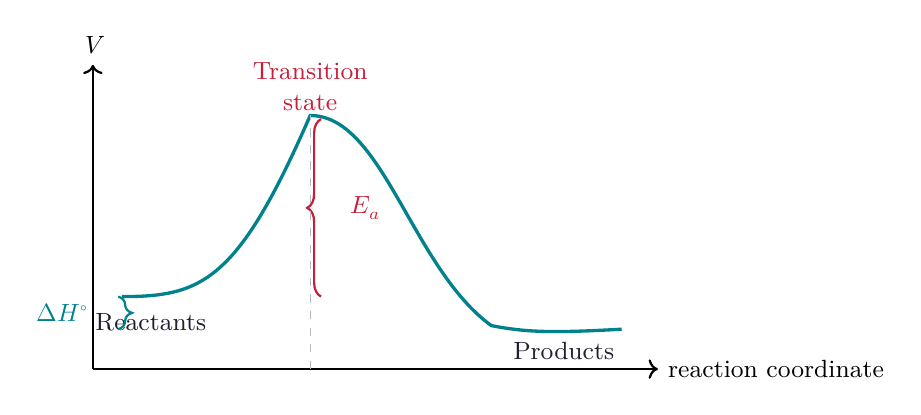
\begin{tikzpicture}[scale=0.92]
  \draw[->, thick] (0,0) -- (7.8,0) node[right, font=\small] {reaction coordinate};
  \draw[->, thick] (0,0) -- (0,4.2) node[above, font=\small] {$V$};
  % energy profile
  \draw[myteal, very thick] (0.4,1.0)
       .. controls (1.5,1.0) and (2.0,1.2) .. (3.0,3.5)
       .. controls (4.0,3.5) and (4.4,1.4) .. (5.5,0.6)
       .. controls (6.0,0.5) and (6.4,0.5) .. (7.3,0.55);
  % reactant/product/TS labels
  \node[font=\small, color=mydark] at (0.8, 0.65) {Reactants};
  \node[font=\small, color=myred,  align=center] at (3.0, 3.9) {Transition\\state};
  \node[font=\small, color=mydark] at (6.5, 0.25) {Products};
  % activation energy brace
  \draw[decorate, decoration={brace, amplitude=5pt}, myred, thick]
       (3.15,1.0) -- (3.15,3.45)
       node[midway, right=7pt, font=\small, color=myred] {$E_a$};
  % delta H brace
  \draw[decorate, decoration={brace, amplitude=5pt, mirror}, myteal, thick]
       (0.35,0.55) -- (0.35,1.0)
       node[midway, left=7pt, font=\small, color=myteal] {$\Delta H^\circ$};
  % dashed vertical at TS
  \draw[dashed, mgframe] (3.0,0) -- (3.0,3.5);
\end{tikzpicture}
\end{tcolorbox}

\textbf{Key features of a PES:}
\begin{itemize}[leftmargin=*, itemsep=2pt, topsep=2pt]
  \item \textbf{Minima} = stable molecules (reactants, products, intermediates).
  \item \textbf{Saddle points} = transition states (highest energy along the reaction path).
  \item \textbf{Activation energy} $E_a$ = energy barrier from reactants to the saddle point.
  \item \textbf{Reaction enthalpy} $\Delta H^\circ$ = difference in energy between reactants and products.
  \item An \emph{exothermic} reaction has products at lower energy; \emph{endothermic} has products higher.
\end{itemize}

\subsection{Transition State Theory (Activated Complex Theory)}
Transition state theory (TST, Eyring, 1935) treats the saddle-point configuration as a quasi-equilibrium ``activated complex'' $[\mathrm{ABC}]^\ddagger$.

\begin{tcolorbox}[formulabox, title={Eyring Rate Equation}]
\[
k = \frac{k_B T}{h}\,e^{-\Delta G^\ddagger/RT} = \frac{k_B T}{h}\,e^{\Delta S^\ddagger/R}\,e^{-\Delta H^\ddagger/RT}
\]
$\Delta G^\ddagger, \Delta H^\ddagger, \Delta S^\ddagger$ are the free energy, enthalpy, and entropy of activation.\\
The factor $k_B T/h \approx 6.3\times10^{12}\ \mathrm{s^{-1}}$ at 298 K is the attempt frequency.
\end{tcolorbox}

\textbf{Connection to Arrhenius:} Comparing with $k=A\,e^{-E_a/RT}$ gives $E_a \approx \Delta H^\ddagger + RT$ and the pre-exponential factor $A = (k_BT/h)\,e^{1+\Delta S^\ddagger/R}$.

\begin{tcolorbox}[exambox, title={Exam Points (Section 2)}]
\begin{itemize}[leftmargin=*, itemsep=2pt, topsep=2pt]
  \item Draw the LJ potential; label $\sigma$, $\varepsilon$, $r_e = 2^{1/6}\sigma$.
  \item At $r_e$: $V$ minimum, $F=0$. For $r<r_e$: repulsion. For $r>r_e$: attraction.
  \item Morse potential adds anharmonicity and dissociation — improves on harmonic oscillator.
  \item On a PES: minima = stable species, saddle points = transition states.
  \item Eyring equation: $k = (k_BT/h)\exp(-\Delta G^\ddagger/RT)$.
\end{itemize}
\end{tcolorbox}

% ===============================================================================
\section{Equations of State for Real Gases}
% ===============================================================================

\begin{tcolorbox}[defbox]
An \textbf{equation of state} (EOS) is a mathematical relationship between the state variables $P$, $V$, $T$, and $n$ of a substance. The ideal gas law ($PV = nRT$) is the simplest EOS but fails at high pressure and low temperature. \emph{Real-gas} equations of state introduce correction terms that account for finite molecular size and intermolecular attractions.
\end{tcolorbox}

\subsection{The Ideal Gas Law and Its Assumptions}
The ideal gas law rests on two assumptions that break down at real conditions:
\begin{enumerate}[leftmargin=*, itemsep=2pt, topsep=2pt]
  \item Molecules are point particles (zero volume).
  \item No intermolecular forces (no attraction or repulsion).
\end{enumerate}

\begin{tcolorbox}[formulabox, title={Ideal Gas Law}]
\[
PV = nRT, \qquad R = 8.314\ \mathrm{J\,mol^{-1}\,K^{-1}} = 0.08206\ \mathrm{L\,atm\,mol^{-1}\,K^{-1}}
\]
\end{tcolorbox}

\subsection{Van der Waals Equation of State}
Van der Waals (1873) introduced two correction parameters:
\begin{itemize}[leftmargin=*, itemsep=2pt, topsep=2pt]
  \item \textbf{$b$ (co-volume):} excluded volume per mole due to finite molecular size. Corrects $V$.
  \item \textbf{$a$ (attraction parameter):} pressure is reduced by attraction, so an internal pressure term $a n^2/V^2$ is added. Corrects $P$.
\end{itemize}

\begin{tcolorbox}[formulabox, title={Van der Waals Equation}]
\[
\boxed{\left(P + \frac{an^2}{V^2}\right)(V - nb) = nRT}
\]
For one mole:
\[
\left(P + \frac{a}{V_m^2}\right)(V_m - b) = RT
\]
$V_m = V/n$ is the molar volume; $a$ in $\mathrm{L^2\,atm\,mol^{-2}}$; $b$ in $\mathrm{L\,mol^{-1}}$.
\end{tcolorbox}

\textbf{Physical interpretation:}
\begin{itemize}[leftmargin=*, itemsep=1pt, topsep=2pt]
  \item $(V_m - b)$: the free volume available to molecules is the total volume minus what the molecules themselves occupy.
  \item $a/V_m^2$: molecules near the wall are pulled back by neighbours --- the measured pressure $P$ is less than the kinetic-theory pressure $P_{\mathrm{kin}}$, so we add back $a/V_m^2$.
\end{itemize}

\begin{tabularx}{\linewidth}{|B{2.4cm}|Y|Y|}
\hline
\textbf{Gas} & \textbf{$a$ (L$^2$ atm mol$^{-2}$)} & \textbf{$b$ (L mol$^{-1}$)} \\
\hline
$\mathrm{H_2}$ & 0.244 & 0.0266 \\
\hline
$\mathrm{N_2}$ & 1.39  & 0.0391 \\
\hline
$\mathrm{CO_2}$ & 3.59 & 0.0427 \\
\hline
$\mathrm{H_2O}$ & 5.46 & 0.0305 \\
\hline
$\mathrm{He}$ & 0.034 & 0.0237 \\
\hline
\end{tabularx}

\begin{tcolorbox}[examplebox, title={Solved Example: Pressure of Real vs Ideal Gas}]
\textbf{Problem:} 1 mol of $\mathrm{CO_2}$ in a $V=1.0\ \mathrm{L}$ container at $T=500\ \mathrm{K}$. Compare ideal and van der Waals pressures.

\textbf{Ideal:}
\[
P_{\mathrm{ideal}} = \frac{RT}{V_m} = \frac{0.08206\times500}{1.0} = 41.0\ \mathrm{atm}
\]
\textbf{Van der Waals} ($a=3.59$, $b=0.0427$):
\[
P = \frac{RT}{V_m - b} - \frac{a}{V_m^2} = \frac{0.08206\times500}{1.0-0.0427} - \frac{3.59}{1.0^2}
= 42.8 - 3.6 = \mathbf{39.2}\ \mathrm{atm}
\]
The real gas pressure is lower because the net effect of attractions ($a$) exceeds the volume correction ($b$) at this condition.
\end{tcolorbox}

\subsection{Compressibility Factor Z}
\begin{tcolorbox}[formulabox, title={Compressibility Factor}]
\[
Z = \frac{PV_m}{RT} = \frac{PV}{nRT}
\]
Ideal gas: $Z = 1$ at all $P$.\\
Real gas: $Z < 1$ when attractions dominate (usually at low--moderate $P$).\\
Real gas: $Z > 1$ when finite volume (repulsion) dominates (very high $P$).
\end{tcolorbox}

\begin{tcolorbox}[tikzbox, title={Compressibility Factor vs Pressure for Real Gases}]
\centering
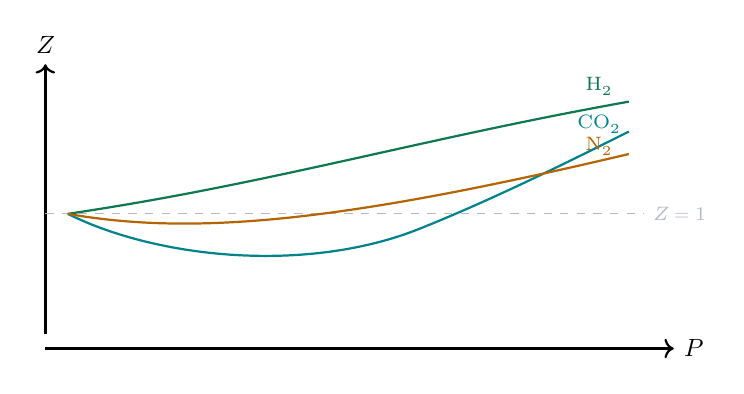
\begin{tikzpicture}[scale=0.95]
  \draw[->, thick] (0,0) -- (8.4,0) node[right, font=\small] {$P$};
  \draw[->, thick] (0,0.2) -- (0,3.8) node[above, font=\small] {$Z$};
  % Z=1 dashed
  \draw[dashed, mgframe] (0.0,1.8) -- (8.0,1.8) node[right, font=\scriptsize] {$Z=1$};
  % H2 (always > 1 at moderate P)
  \draw[mygreen, thick] (0.3,1.8) .. controls (3,2.2) and (5,2.8) .. (7.8,3.3);
  \node[mygreen, font=\scriptsize] at (7.4,3.5) {$\mathrm{H_2}$};
  % CO2 (dips below then rises)
  \draw[myteal, thick] (0.3,1.8) .. controls (1.5,1.2) and (3.5,1.0) .. (5.0,1.6)
       .. controls (6.0,2.0) and (7.0,2.5) .. (7.8,2.9);
  \node[myteal, font=\scriptsize] at (7.4,3.0) {$\mathrm{CO_2}$};
  % N2
  \draw[myamber, thick] (0.3,1.8) .. controls (2.0,1.5) and (4.0,1.7) .. (7.8,2.6);
  \node[myamber, font=\scriptsize] at (7.4,2.7) {$\mathrm{N_2}$};
\end{tikzpicture}
\end{tcolorbox}

\subsection{Virial Equation of State}
The virial equation expresses $Z$ as a power series in density $1/V_m$:

\begin{tcolorbox}[formulabox, title={Virial Equation of State}]
\[
Z = \frac{PV_m}{RT} = 1 + \frac{B}{V_m} + \frac{C}{V_m^2} + \cdots
\]
$B$ = second virial coefficient (accounts for pair interactions), $C$ = third virial coefficient. For the van der Waals gas at low density: $B = b - a/(RT)$.\\
At the Boyle temperature $T_B$: $B = 0$ so $Z \approx 1$ at low--moderate pressure.
\end{tcolorbox}

\subsection{Other Equations of State}

\begin{tabularx}{\linewidth}{|B{2.6cm}|Y|Y|}
\hline
\textbf{EOS} & \textbf{Expression (1 mol)} & \textbf{Improvement over VdW} \\
\hline
Dieterici & $P(V_m-b)=RT\,e^{-a/RTV_m}$ & Better near critical point \\
\hline
Redlich--Kwong & $P=\displaystyle\frac{RT}{V_m-b}-\frac{a}{T^{1/2}V_m(V_m+b)}$ & Better for gas-phase calculations \\
\hline
Peng--Robinson & Modified cubic with two parameters & Used in petroleum engineering \\
\hline
Ideal gas & $PV_m = RT$ & Reference baseline \\
\hline
\end{tabularx}

\subsection{Boyle Temperature}
At the Boyle temperature, the second virial coefficient $B = 0$, so the gas behaves nearly ideally over a range of pressures.

\begin{tcolorbox}[formulabox, title={Boyle Temperature for a van der Waals Gas}]
\[
T_B = \frac{a}{Rb}
\]
\end{tcolorbox}

\begin{tcolorbox}[examplebox, title={Solved Example: Boyle Temperature of \texorpdfstring{$\mathrm{CO_2}$}{CO2}}]
$a=3.59\ \mathrm{L^2\,atm\,mol^{-2}}$, $b=0.0427\ \mathrm{L\,mol^{-1}}$:
\[
T_B = \frac{3.59}{0.08206\times0.0427} = \frac{3.59}{0.003504} = 1024\ \mathrm{K}
\]
Below $T_B$ (1024 K for $\mathrm{CO_2}$), attractions dominate and $Z<1$ at modest pressures.
\end{tcolorbox}

\subsection{Joule--Thomson Effect}
When a real gas expands irreversibly through a porous plug (throttle) from high pressure to low, the process is isenthalpic ($\Delta H = 0$). The temperature may rise or fall.

\begin{tcolorbox}[formulabox, title={Joule--Thomson Coefficient}]
\[
\mu_{\mathrm{JT}} = \left(\frac{\partial T}{\partial P}\right)_H
\]
For a van der Waals gas at low density:
\[
\mu_{\mathrm{JT}} \approx \frac{1}{C_P}\!\left(\frac{2a}{RT} - b\right)
\]
\textbf{At $T < T_i$ (inversion temperature):} $\mu_{\mathrm{JT}} > 0$, gas cools on expansion.\\
\textbf{At $T > T_i$:} $\mu_{\mathrm{JT}} < 0$, gas warms on expansion.
\end{tcolorbox}

\begin{tabularx}{\linewidth}{|B{3.0cm}|Y|Y|}
\hline
\textbf{Condition} & \textbf{$\mu_{\mathrm{JT}}$} & \textbf{Effect} \\
\hline
$T < T_i$ & Positive & Cooling (used in liquefaction) \\
\hline
$T = T_i$ & Zero & No temperature change \\
\hline
$T > T_i$ & Negative & Heating \\
\hline
\end{tabularx}

\textbf{Inversion temperature:} $T_i = 2a/(Rb)$. Note $T_i = 2T_B$. For $\mathrm{N_2}$: $T_i\approx 621\ \mathrm{K}$, so pre-cooling is needed before throttling to liquefy nitrogen. For $\mathrm{H_2}$ and $\mathrm{He}$: $T_i$ is below room temperature, so they warm on throttling without pre-cooling.

\begin{tcolorbox}[masonbox, title={Linde Liquefaction Process and Joule--Thomson Effect}]
The Linde process uses the Joule--Thomson effect to liquefy air: compressed gas expands through a throttle valve, cools, is recycled back, and after many cycles reaches the liquefaction temperature. Gas must be pre-cooled below its inversion temperature first. This principle is used to produce liquid $\mathrm{N_2}$ ($77\ \mathrm{K}$), liquid $\mathrm{O_2}$ ($90\ \mathrm{K}$), and liquid air for cryogenics.
\end{tcolorbox}

\begin{tcolorbox}[exambox, title={Exam Points (Section 3)}]
\begin{itemize}[leftmargin=*, itemsep=2pt, topsep=2pt]
  \item Van der Waals: $a$ corrects $P$ (attractions), $b$ corrects $V$ (molecular size).
  \item Solve $P = RT/(V_m-b) - a/V_m^2$ numerically in 5-mark problems.
  \item $Z < 1$: attraction-dominated; $Z > 1$: repulsion-dominated.
  \item Boyle temperature: $T_B = a/(Rb)$; $B = 0$ there.
  \item Joule--Thomson: isenthalpic expansion; $\mu_{\mathrm{JT}} > 0$ below inversion temperature.
  \item Inversion temperature: $T_i = 2a/(Rb) = 2T_B$.
\end{itemize}
\end{tcolorbox}

% ===============================================================================
\section{Critical Phenomena and the Continuity of State}
% ===============================================================================

\begin{tcolorbox}[defbox]
\textbf{Critical phenomena} describe the behaviour of substances at the \emph{critical point} --- the unique temperature $T_c$, pressure $P_c$, and molar volume $V_c$ at which the liquid--vapour interface vanishes and liquid and vapour become identical. Above $T_c$, no amount of pressure can liquefy the gas.
\end{tcolorbox}

\subsection{Phase Diagram and the Liquid--Vapour Boundary}

\begin{tcolorbox}[tikzbox, title={Pressure--Temperature Phase Diagram}]
\centering
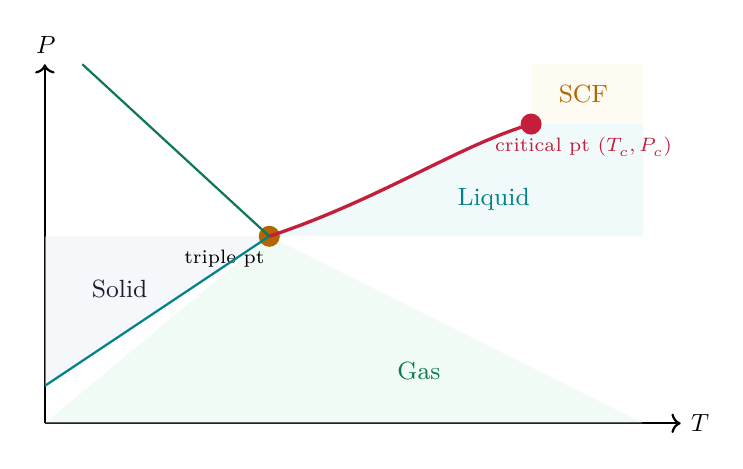
\begin{tikzpicture}[scale=0.95]
  \draw[->, thick] (0,0) -- (8.5,0) node[right, font=\small] {$T$};
  \draw[->, thick] (0,0) -- (0,4.8) node[above, font=\small] {$P$};
  % Solid region
  \fill[hdrgray, opacity=0.5] (0,0.5)--(3.0,2.5)--(0,2.5)--cycle;
  \node[font=\small, color=mydark] at (1.0,1.8) {Solid};
  % Liquid region
  \fill[hdrteal, opacity=0.4] (3.0,2.5)--(6.5,4.0)--(8.0,4.0)--(8.0,2.5)--cycle;
  \node[font=\small, color=myteal] at (6.0,3.0) {Liquid};
  % Gas region
  \fill[hdrgreen, opacity=0.4] (0,0)--(3.0,2.5)--(8.0,0)--cycle;
  \node[font=\small, color=mygreen] at (5.0,0.7) {Gas};
  % Supercritical
  \fill[hdramber, opacity=0.3] (6.5,4.0)--(8.0,4.0)--(8.0,4.8)--(6.5,4.8)--cycle;
  \node[font=\small, color=myamber] at (7.2,4.4) {SCF};
  % Triple point
  \fill[myamber] (3.0,2.5) circle (4pt);
  \node[font=\scriptsize] at (2.4,2.2) {triple pt};
  % Critical point
  \fill[myred] (6.5,4.0) circle (4pt);
  \node[font=\scriptsize, color=myred] at (7.2,3.7) {critical pt ($T_c,P_c$)};
  % Vapour pressure curve
  \draw[myred, very thick] (3.0,2.5) .. controls (4.5,3.0) and (5.5,3.7) .. (6.5,4.0);
  % Sublimation and fusion curves
  \draw[myteal, thick] (3.0,2.5) -- (0,0.5);
  \draw[mygreen, thick] (3.0,2.5) -- (0.5,4.8);
\end{tikzpicture}
\end{tcolorbox}

\textbf{Key points:}
\begin{itemize}[leftmargin=*, itemsep=1pt, topsep=2pt]
  \item \textbf{Triple point}: all three phases coexist (unique $T$ and $P$). For water: $T_{tr}=273.16\ \mathrm{K}$, $P_{tr}=611.7\ \mathrm{Pa}$.
  \item \textbf{Critical point}: liquid--vapour boundary terminates. Above $T_c$: single supercritical fluid (SCF) phase.
  \item \textbf{Vapour pressure curve}: slope given by Clausius--Clapeyron equation.
\end{itemize}

\subsection{Derivation of Critical Constants from the Van der Waals Equation}

\begin{tcolorbox}[formulabox, title={Conditions at the Critical Point}]
At the critical point, the isotherm has an inflection point with zero slope:
\[
\left(\frac{\partial P}{\partial V_m}\right)_{T_c} = 0
\qquad\text{and}\qquad
\left(\frac{\partial^2 P}{\partial V_m^2}\right)_{T_c} = 0
\]
\end{tcolorbox}

Starting from the van der Waals EOS for 1 mol:
\[
P = \frac{RT}{V_m - b} - \frac{a}{V_m^2}
\]

First derivative:
\[
\frac{\partial P}{\partial V_m} = -\frac{RT}{(V_m-b)^2} + \frac{2a}{V_m^3} = 0
\quad\Rightarrow\quad RT(V_m-b)^2 = 2a\,\frac{(V_m-b)^2\,(V_m-b)}{V_m^3}\cdot V_m^3 \tag{i}
\]

Second derivative:
\[
\frac{\partial^2 P}{\partial V_m^2} = \frac{2RT}{(V_m-b)^3} - \frac{6a}{V_m^4} = 0
\quad\Rightarrow\quad RT(V_m-b)^3 = 3a\cdot\frac{(V_m-b)^3}{V_m^4}\cdot V_m^4 \tag{ii}
\]

Dividing (ii) by (i):
\[
\frac{(V_m-b)}{1} = \frac{3}{2}V_m \quad\Rightarrow\quad 2V_m - 2b = 3V_m \quad\Rightarrow\quad \boxed{V_c = 3b}
\]

Substituting back into (i):
\[
RT_c = \frac{2a(V_c-b)^2}{V_c^3} = \frac{2a(2b)^2}{(3b)^3} = \frac{8a}{27b}
\quad\Rightarrow\quad \boxed{T_c = \frac{8a}{27Rb}}
\]

And using the VdW EOS at the critical point:
\[
\boxed{P_c = \frac{a}{27b^2}}
\]

\begin{tcolorbox}[formulabox, title={Critical Constants (Van der Waals)}]
\[
V_c = 3b, \qquad T_c = \frac{8a}{27Rb}, \qquad P_c = \frac{a}{27b^2}
\]
Also useful: $\displaystyle\frac{P_c V_c}{RT_c} = \frac{3}{8} = 0.375$\quad (critical compression factor for a VdW gas).
\end{tcolorbox}

\begin{tcolorbox}[examplebox, title={Solved Example: Critical Constants of \texorpdfstring{$\mathrm{N_2}$}{N2}}]
$a=1.39\ \mathrm{L^2\,atm\,mol^{-2}}$, $b=0.0391\ \mathrm{L\,mol^{-1}}$:
\[
V_c = 3(0.0391) = 0.117\ \mathrm{L\,mol^{-1}}
\]
\[
T_c = \frac{8(1.39)}{27(0.08206)(0.0391)} = \frac{11.12}{0.08661} = 128.4\ \mathrm{K}
\]
\[
P_c = \frac{1.39}{27(0.0391)^2} = \frac{1.39}{0.04128} = 33.7\ \mathrm{atm}
\]
Experimental: $T_c=126.2\ \mathrm{K}$, $P_c=33.9\ \mathrm{atm}$ --- excellent agreement.
\end{tcolorbox}

\subsection{Reduced Variables and the Law of Corresponding States}

\begin{tcolorbox}[defbox]
\textbf{Reduced variables} express $T$, $P$, and $V$ as fractions of their critical values:
\[
T_r = \frac{T}{T_c}, \qquad P_r = \frac{P}{P_c}, \qquad V_r = \frac{V_m}{V_c}
\]
\textbf{Law of Corresponding States (van der Waals):} All gases obey the \emph{same} equation of state when expressed in terms of reduced variables, regardless of their identity.
\end{tcolorbox}

Substituting into the van der Waals equation:
\[
\left(P_r + \frac{3}{V_r^2}\right)\!\left(V_r - \frac{1}{3}\right) = \frac{8}{3}T_r
\]
This \emph{reduced van der Waals equation} has no gas-specific parameters. It predicts that at the same $T_r$ and $P_r$, all gases have the same $Z$ --- the basis of \emph{generalised compressibility charts} used in engineering.

\begin{tcolorbox}[examplebox, title={Application: Comparing States of Different Gases}]
$\mathrm{CO_2}$ at $T=340\ \mathrm{K}$, $P=100\ \mathrm{atm}$ has $T_r=340/304=1.12$ and $P_r=100/72.9=1.37$.\\
$\mathrm{CH_4}$ at $T=215\ \mathrm{K}$, $P=63.5\ \mathrm{atm}$ has $T_r=215/191=1.12$ and $P_r=63.5/46.1=1.38$.\\
By the law of corresponding states, both gases have approximately the same $Z$ even though their absolute conditions differ.
\end{tcolorbox}

\subsection{Andrews Isotherms and the Critical Region}

\begin{tcolorbox}[tikzbox, title={$P$--$V_m$ Isotherms of a Real Gas (Andrews-Type)}]
\centering
\begin{tikzpicture}[scale=0.95]
  \draw[->, thick] (0,0) -- (8.5,0) node[right, font=\small] {$V_m$};
  \draw[->, thick] (0,0) -- (0,4.8) node[above, font=\small] {$P$};
  % Isotherm T >> Tc (nearly ideal)
  \draw[mygreen, thick, domain=1.0:8.0, smooth, variable=\x]
       plot (\x, {3.0/\x+0.3}) node[right, font=\scriptsize, color=mygreen] {$T \gg T_c$};
  % Isotherm T > Tc
  \draw[myteal, thick, domain=0.8:8.0, smooth, variable=\x]
       plot (\x, {2.0/\x+0.15}) node[right, font=\scriptsize, color=myteal] {$T > T_c$};
  % Critical isotherm
  \draw[myred, very thick, domain=0.65:8.0, smooth, variable=\x]
       plot (\x, {2.9*exp(-0.6*(\x-1.5))^3 - 1.0*exp(-0.3*(\x-1.5))+1.2})
       node[right, font=\scriptsize, color=myred] {$T = T_c$};
  % Critical point
  \fill[myred] (1.5,1.2) circle (4pt);
  \node[myred, font=\scriptsize, anchor=south] at (1.8,1.4) {CP};
  % Subcritical isotherm with horizontal portion
  \draw[mypurple, thick] (0.5,2.5)--(0.8,2.5);
  \draw[mypurple, thick] (0.8,2.5) -- (4.2,2.5);
  \draw[mypurple, thick] (4.2,2.5)--(4.2,0.6);
  \draw[mypurple, thick, domain=4.2:8.0, smooth, variable=\x]
       plot (\x, {0.6/(\x-0.1)+0.1});
  \node[mypurple, font=\scriptsize] at (2.5,2.8) {$T < T_c$ (two-phase)};
\end{tikzpicture}
\end{tcolorbox}

\textbf{Reading the isotherms:}
\begin{itemize}[leftmargin=*, itemsep=2pt, topsep=2pt]
  \item Above $T_c$: smooth curves, gas cannot be liquefied.
  \item At $T_c$: inflection point at the critical point (critical isotherm).
  \item Below $T_c$: isotherms show a \emph{horizontal portion} where liquid and vapour coexist at constant $P$ (vapour pressure). Compression reduces volume along this plateau until all vapour condenses.
\end{itemize}

\subsection{Clausius--Clapeyron Equation}
Along the vapour-pressure curve, the slope $dP/dT$ is given by the Clausius--Clapeyron equation.

\begin{tcolorbox}[formulabox, title={Clausius--Clapeyron Equation}]
\[
\frac{dP}{dT} = \frac{\Delta H_{\mathrm{vap}}}{T\,\Delta V_{\mathrm{vap}}}
\quad\xrightarrow{\text{ideal gas approx.}}\quad
\frac{d\ln P}{dT} = \frac{\Delta H_{\mathrm{vap}}}{RT^2}
\]
Integrated form:
\[
\ln\frac{P_2}{P_1} = -\frac{\Delta H_{\mathrm{vap}}}{R}\!\left(\frac{1}{T_2}-\frac{1}{T_1}\right)
\]
A plot of $\ln P$ vs $1/T$ is linear with slope $-\Delta H_{\mathrm{vap}}/R$.
\end{tcolorbox}

\begin{tcolorbox}[examplebox, title={Solved Example: Vapour Pressure of Water}]
Water has $\Delta H_{\mathrm{vap}}=40.7\ \mathrm{kJ\,mol^{-1}}$. At $T_1=373\ \mathrm{K}$, $P_1=1\ \mathrm{atm}$. Find $P$ at $T_2=393\ \mathrm{K}$.
\[
\ln\frac{P_2}{1} = -\frac{40700}{8.314}\!\left(\frac{1}{393}-\frac{1}{373}\right)
= -4893\times(-1.364\times10^{-4}) = 0.668
\]
\[
P_2 = e^{0.668} = 1.95\ \mathrm{atm}
\]
The vapour pressure nearly doubles from $373\ \mathrm{K}$ to $393\ \mathrm{K}$, consistent with the rapid increase seen in pressure cookers.
\end{tcolorbox}

\subsection{Supercritical Fluids}
Above $T_c$ and $P_c$ the distinction between liquid and gas vanishes. The substance is a \textbf{supercritical fluid (SCF)} with properties intermediate between liquid and gas.

\begin{tabularx}{\linewidth}{|B{2.6cm}|Y|Y|Y|}
\hline
\textbf{Property} & \textbf{Gas} & \textbf{SCF} & \textbf{Liquid} \\
\hline
Density & Low & Liquid-like & High \\
\hline
Diffusivity & High & Intermediate & Low \\
\hline
Viscosity & Low & Low & High \\
\hline
Solvation & Negligible & Tunable & Fixed \\
\hline
\end{tabularx}

\textbf{Critical constants of common SCF solvents:}\par\noindent
\begin{tabularx}{\linewidth}{|B{2.4cm}|Y|Y|Y|}
\hline
\textbf{Solvent} & \textbf{$T_c$ (K)} & \textbf{$P_c$ (bar)} & \textbf{Applications} \\
\hline
$\mathrm{CO_2}$ & 304 & 73.8 & Decaffeination, dry cleaning, drug extraction \\
\hline
$\mathrm{H_2O}$ & 647 & 220.9 & Oxidation of organic waste, hydrothermal synthesis \\
\hline
$\mathrm{CH_4}$ & 191 & 46.1 & Natural gas processing \\
\hline
Ethanol & 516 & 63.8 & Food industry extraction \\
\hline
\end{tabularx}

\begin{tcolorbox}[masonbox, title={Why \texorpdfstring{$\mathrm{sc}$-$\mathrm{CO_2}$}{sc-CO2} is the Industrial SCF of Choice}]
Supercritical $\mathrm{CO_2}$ has $T_c=304\ \mathrm{K}$ (near room temperature) and $P_c=73.8\ \mathrm{bar}$ (accessible with standard pumps). It is non-toxic, non-flammable, cheap, and leaves no solvent residue. Its solvating power is tunable by pressure, making it ideal for pharmaceutical extraction, polymer processing, and green chemistry.
\end{tcolorbox}

\begin{tcolorbox}[exambox, title={Exam Points (Section 4)}]
\begin{itemize}[leftmargin=*, itemsep=2pt, topsep=2pt]
  \item Derive $V_c=3b$, $T_c=8a/27Rb$, $P_c=a/27b^2$ from the VdW conditions at CP.
  \item Critical compression factor: $Z_c = P_cV_c/RT_c = 3/8$.
  \item Law of corresponding states: all gases follow the same reduced VdW EOS.
  \item Andrews isotherms: identify two-phase region, critical point, and supercritical region.
  \item Clausius--Clapeyron: $\ln(P_2/P_1) = -(\Delta H_{\mathrm{vap}}/R)(1/T_2 - 1/T_1)$.
  \item SCF properties: liquid-like density, gas-like diffusivity; CO$_2$ example.
\end{itemize}
\end{tcolorbox}

% ===============================================================================
\section{Applications of Intermolecular Forces and Real-Gas Behaviour}
% ===============================================================================

\begin{tcolorbox}[defbox]
Understanding IMFs and real-gas equations of state is not purely theoretical --- they govern physical properties and underpin industrial processes from gas liquefaction to drug design.
\end{tcolorbox}

\subsection{Effect of IMFs on Physical Properties}

\begin{tabularx}{\linewidth}{|B{3.0cm}|Y|Y|}
\hline
\textbf{Property} & \textbf{How IMF controls it} & \textbf{Example} \\
\hline
Boiling point & Stronger IMF $\Rightarrow$ more energy to vaporise & $\mathrm{H_2O}$ (100$^\circ$C) vs $\mathrm{H_2S}$ ($-60^\circ$C) \\
\hline
Melting point & Stronger crystal forces $\Rightarrow$ higher mp & NaCl (801$^\circ$C) vs Ar ($-189^\circ$C) \\
\hline
Viscosity & Larger/polar molecules have stronger IMF $\Rightarrow$ more resistance to flow & Glycerol $\gg$ water \\
\hline
Surface tension & IMF pulling surface molecules inward & Water (72 mN m$^{-1}$) $\gg$ hexane (18 mN m$^{-1}$) \\
\hline
Solubility & Like-dissolves-like: matching IMF types & NaCl in water, iodine in CCl$_4$ \\
\hline
Heat of vaporisation & Energy to overcome IMF & Water $44\ \mathrm{kJ\,mol^{-1}}$, hexane $31\ \mathrm{kJ\,mol^{-1}}$ \\
\hline
\end{tabularx}

\subsection{Like-Dissolves-Like Rule}
\begin{tcolorbox}[defbox]
\textbf{Like dissolves like:} A solute dissolves in a solvent when the solvent--solute interactions are comparable in type and strength to the solvent--solvent interactions. Polar solutes dissolve in polar solvents; non-polar solutes dissolve in non-polar solvents.
\end{tcolorbox}

\textbf{Thermodynamic justification:} Dissolution is spontaneous when $\Delta G_{\mathrm{solvation}} < 0$. This requires $\Delta H_{\mathrm{solvation}} \approx -(\Delta H_{\mathrm{lattice/assoc}} + \Delta H_{\mathrm{solvent\ cavity}})$, which holds when IMF types match.

\subsection{Hydrogen Bonding in Biological Systems}
\begin{itemize}[leftmargin=*, itemsep=2pt, topsep=2pt]
  \item \textbf{DNA base pairing:} A--T has 2 H-bonds ($20\ \mathrm{kJ\,mol^{-1}}$); G--C has 3 ($30\ \mathrm{kJ\,mol^{-1}}$). Collectively they stabilise the double helix.
  \item \textbf{Protein folding:} H-bonds between backbone N--H and C$=$O groups stabilise $\alpha$-helices and $\beta$-sheets.
  \item \textbf{Enzyme catalysis:} H-bonds in the active site position substrates precisely.
  \item \textbf{Membrane fluidity:} Phospholipid bilayers rely on London forces between non-polar tails, H-bonds between polar heads and water.
\end{itemize}

\subsection{Gas Liquefaction and Industrial Gases}
Liquefying a gas requires cooling it below its critical temperature and then compressing it. The Joule--Thomson effect is harnessed industrially.

\begin{tcolorbox}[tikzbox, title={Linde Liquefaction Cycle (Schematic)}]
\centering
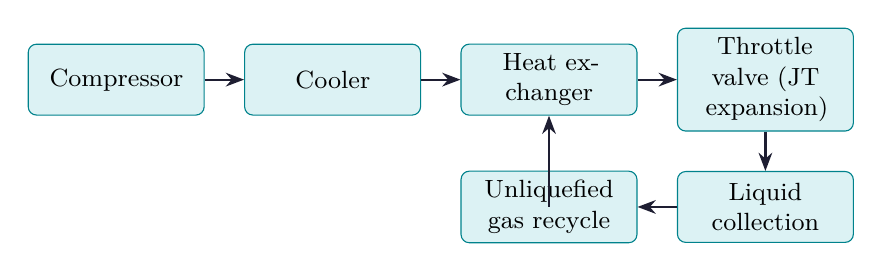
\begin{tikzpicture}[node distance=0.3cm and 0.4cm,
  sblock/.style={rectangle, draw=myteal, fill=hdrteal, text width=2.0cm,
    align=center, minimum height=0.9cm, font=\small, rounded corners=3pt}]
  \node[sblock] (n1) {Compressor};
  \node[sblock, right=0.5cm of n1] (n2) {Cooler};
  \node[sblock, right=0.5cm of n2] (n3) {Heat exchanger};
  \node[sblock, right=0.5cm of n3] (n4) {Throttle valve (JT expansion)};
  \node[sblock, below=0.5cm of n4] (n5) {Liquid collection};
  \node[sblock, left=0.5cm of n5] (n6) {Unliquefied gas recycle};
  \draw[arrow] (n1)--(n2);
  \draw[arrow] (n2)--(n3);
  \draw[arrow] (n3)--(n4);
  \draw[arrow] (n4)--(n5);
  \draw[arrow] (n5)--(n6);
  \draw[arrow] (n6)-|(n3);
\end{tikzpicture}
\end{tcolorbox}

\textbf{Industrial cryogens and their $T_c$:}
\begin{itemize}[leftmargin=*, itemsep=1pt, topsep=2pt]
  \item Liquid $\mathrm{N_2}$ ($77\ \mathrm{K}$): $T_c=126\ \mathrm{K}$, pre-cooling to $\sim100\ \mathrm{K}$ needed.
  \item Liquid $\mathrm{O_2}$ ($90\ \mathrm{K}$): $T_c=155\ \mathrm{K}$.
  \item Liquid $\mathrm{He}$ ($4.2\ \mathrm{K}$): $T_c=5.2\ \mathrm{K}$, requires liquid $\mathrm{N_2}$ pre-cool then JT expansion.
  \item Liquid $\mathrm{H_2}$ ($20\ \mathrm{K}$): $T_c=33\ \mathrm{K}$, must pre-cool below inversion temperature.
\end{itemize}

\subsection{Real Gases in Engineering Calculations}
Van der Waals and virial equations are used in:
\begin{itemize}[leftmargin=*, itemsep=1pt, topsep=2pt]
  \item Pipeline sizing for high-pressure natural gas ($Z\neq1$).
  \item Refrigeration cycle analysis (refrigerant properties near $T_c$).
  \item Supercritical extraction unit design.
  \item Prediction of dew points and bubble points in process engineering.
\end{itemize}

\subsection{Colligative Properties: IMF Context}
Though formally under solution chemistry, colligative properties arise from the modification of solvent--solvent IMFs by added solute.

\begin{tabularx}{\linewidth}{|B{3.0cm}|Y|Y|}
\hline
\textbf{Property} & \textbf{IMF connection} & \textbf{Equation} \\
\hline
Boiling-point elevation & Solute lowers solvent vapour pressure $\Rightarrow$ higher bp & $\Delta T_b = K_b\,m$ \\
\hline
Freezing-point depression & Solute disrupts lattice IMF network & $\Delta T_f = K_f\,m$ \\
\hline
Osmotic pressure & Solute concentration drives solvent flow across membrane & $\pi = iMRT$ \\
\hline
Raoult's law & Vapour pressure lowering $\Delta P = x_{\mathrm{sol}}P^\circ$ & Based on ideal mixing of IMFs \\
\hline
\end{tabularx}

\begin{tcolorbox}[exambox, title={Exam Points (Section 5)}]
\begin{itemize}[leftmargin=*, itemsep=2pt, topsep=2pt]
  \item Boiling point order: relates directly to IMF strength (H-bond $>$ dipole $>$ London).
  \item Like-dissolves-like: IMF type determines solubility.
  \item DNA A--T: 2 H-bonds; G--C: 3 H-bonds --- explains higher $T_m$ of GC-rich DNA.
  \item Linde process: compressor $\to$ cooler $\to$ heat exchanger $\to$ throttle (JT cooling) $\to$ liquid.
  \item Clausius--Clapeyron gives slope of vapour-pressure curve; use to find $\Delta H_{\mathrm{vap}}$.
\end{itemize}
\end{tcolorbox}

% ===============================================================================
\newpage
\begin{center}
  {\large\bfseries\color{myred} Quick Revision --- Module 3}\\[3pt]
  {\small\color{mydark} Intermolecular Forces, Real Gases and Critical Phenomena $|$ BS-CH101}
\end{center}
\noindent{\color{myred}\rule{\linewidth}{1.2pt}}
\vspace{4pt}

\begin{tcolorbox}[formulabox, breakable, title={Key Formulas at a Glance},
  title after break={\textbf{Key Formulas at a Glance (contd.)}}]
{\renewcommand{\arraystretch}{1.55}
\begin{tabularx}{\linewidth}{|B{4.6cm}|Y|}
\hline
\textbf{Formula} & \textbf{Meaning} \\
\hline
$V_{\mathrm{ion-ion}} = -\displaystyle\frac{z_1 z_2 e^2}{4\pi\varepsilon_0 r}$ & Coulomb energy between two ions ($\propto r^{-1}$). \\
\hline
$\mu = q\cdot d$ & Dipole moment; 1 D $= 3.336\times10^{-30}\ \mathrm{C\,m}$. \\
\hline
$V_{\mathrm{Keesom}} \propto -\displaystyle\frac{\mu^4}{k_BT\,r^6}$ & Dipole--dipole (thermal-averaged); $r^{-6}$, $T$-dependent. \\
\hline
$V_{\mathrm{London}} \propto -\displaystyle\frac{\alpha_1'\alpha_2' I_1 I_2}{r^6(I_1+I_2)}$ & London dispersion; $r^{-6}$, $T$-independent. \\
\hline
$V_{\mathrm{LJ}} = 4\varepsilon\!\left[(\sigma/r)^{12}-(\sigma/r)^6\right]$ & Lennard-Jones 12-6 potential; $r_e=2^{1/6}\sigma$. \\
\hline
$F = -dV/dr$ & Force from potential energy curve. \\
\hline
$V_{\mathrm{Morse}} = D_e[1-e^{-\beta(r-r_e)}]^2$ & Morse bond potential with dissociation limit. \\
\hline
$\left(P+\displaystyle\frac{a}{V_m^2}\right)(V_m-b)=RT$ & Van der Waals EOS (one mole). \\
\hline
$Z = PV_m/RT$ & Compressibility factor; $Z=1$ ideal. \\
\hline
$Z = 1 + B/V_m + C/V_m^2 + \cdots$ & Virial EOS; $B = b - a/(RT)$ for VdW. \\
\hline
\end{tabularx}}
\vspace{3pt}
{\renewcommand{\arraystretch}{1.55}
\begin{tabularx}{\linewidth}{|B{4.6cm}|Y|}
\hline
$T_B = a/(Rb)$ & Boyle temperature ($B=0$, near-ideal). \\
\hline
$V_c = 3b$, $T_c = 8a/27Rb$, $P_c = a/27b^2$ & Critical constants (VdW). \\
\hline
$Z_c = P_cV_c/RT_c = 3/8$ & Critical compressibility factor (VdW). \\
\hline
$T_r = T/T_c$, $P_r = P/P_c$, $V_r = V_m/V_c$ & Reduced variables. \\
\hline
$(P_r+3/V_r^2)(V_r-1/3)=8T_r/3$ & Reduced VdW EOS (universal). \\
\hline
$\mu_{\mathrm{JT}} = (\partial T/\partial P)_H$ & Joule--Thomson coefficient. \\
\hline
$T_i = 2a/(Rb) = 2T_B$ & Inversion temperature. \\
\hline
$\ln(P_2/P_1)=-(\Delta H_{\mathrm{vap}}/R)(1/T_2 - 1/T_1)$ & Clausius--Clapeyron (integrated). \\
\hline
$\Delta T_b = K_b m$; $\Delta T_f = K_f m$; $\pi = iMRT$ & Colligative properties. \\
\hline
\end{tabularx}}
\end{tcolorbox}

\begin{tcolorbox}[defbox, title={One-Line Definitions}]
\begin{itemize}[leftmargin=*, itemsep=2pt, topsep=2pt]
  \item \textbf{Intermolecular force:} Attractive or repulsive force between separate molecules/ions.
  \item \textbf{Dipole moment:} Vector quantity $\mu = qd$; non-zero for asymmetric charge distribution.
  \item \textbf{London dispersion:} IMF due to instantaneous and induced temporary dipoles; exists in all molecules.
  \item \textbf{Keesom interaction:} Thermal-averaged attraction between two permanent dipoles; proportional to $r^{-6}$ and $1/T$.
  \item \textbf{Debye interaction:} Attraction of permanent dipole on an induced dipole; $r^{-6}$, temperature-independent.
  \item \textbf{Hydrogen bond:} Strong directional interaction of H (bonded to F/O/N) with a lone pair; $15$--$40\ \mathrm{kJ\,mol^{-1}}$.
  \item \textbf{Polarisability:} Ease of distortion of an electron cloud by an electric field; increases down a group.
  \item \textbf{Lennard-Jones potential:} Empirical 12-6 pair potential combining repulsion and London dispersion.
  \item \textbf{Equilibrium separation ($r_e$):} Distance at which $V$ is minimum and $F = 0$.
  \item \textbf{Potential energy surface:} Multi-dimensional energy landscape as function of molecular geometry.
  \item \textbf{Transition state:} Saddle point on the PES; highest energy along the reaction path.
  \item \textbf{Activation energy ($E_a$):} Energy barrier separating reactants from transition state.
  \item \textbf{Real gas:} Gas deviating from ideal due to finite molecular volume and attractions.
  \item \textbf{Van der Waals $a$:} Correction for intermolecular attractions (reduces pressure).
  \item \textbf{Van der Waals $b$:} Excluded volume per mole due to finite molecular size (reduces free volume).
  \item \textbf{Compressibility factor ($Z$):} $PV_m/RT$; equals 1 for ideal gas.
  \item \textbf{Virial coefficient $B$:} Second virial coefficient; zero at Boyle temperature.
  \item \textbf{Boyle temperature:} $T_B = a/(Rb)$; gas behaves nearly ideally.
  \item \textbf{Critical temperature ($T_c$):} Highest $T$ at which gas can be liquefied by pressure alone.
  \item \textbf{Critical pressure ($P_c$):} Pressure needed to liquefy gas at $T_c$.
  \item \textbf{Critical point:} State where liquid and vapour become identical; $(T_c, P_c, V_c)$.
  \item \textbf{Reduced variables:} $T_r$, $P_r$, $V_r$; enable law of corresponding states.
  \item \textbf{Law of corresponding states:} All gases obey the same reduced EOS.
  \item \textbf{Joule--Thomson effect:} Temperature change of real gas on isenthalpic expansion through a throttle.
  \item \textbf{Inversion temperature ($T_i$):} $\mu_{\mathrm{JT}} = 0$; $T_i = 2a/(Rb)$.
  \item \textbf{Supercritical fluid:} Phase above $T_c$ and $P_c$ with liquid-like density and gas-like diffusivity.
  \item \textbf{Clausius--Clapeyron equation:} Relates vapour pressure change to temperature via $\Delta H_{\mathrm{vap}}$.
  \item \textbf{Like-dissolves-like:} Solubility is maximised when solute--solvent IMF type matches.
  \item \textbf{Linde process:} Industrial gas liquefaction using Joule--Thomson expansion cycle.
\end{itemize}
\end{tcolorbox}

\begin{tcolorbox}[exambox, title={Frequently Asked / Viva Questions}]
\begin{enumerate}[topsep=0pt, label=\textbf{Q\arabic*.}, itemsep=5pt]
  \item \Q{What are intermolecular forces? Arrange them in increasing strength.}
    Forces between molecules/ions: London $<$ dipole--dipole $<$ H-bond $<$ ion--dipole $<$ ion--ion.
  \item \Q{Why do London forces increase down a noble-gas group?}
    Larger atoms have more electrons and higher polarisability; instantaneous dipoles are stronger.
  \item \Q{Why is $\mathrm{CO_2}$ non-polar despite having polar bonds?}
    Linear geometry makes bond-dipole vectors cancel exactly.
  \item \Q{What is Keesom interaction and why is it temperature-dependent?}
    Dipole--dipole orientation averaged over thermal motion; higher $T$ scrambles alignment, weakening the interaction.
  \item \Q{State the Lennard-Jones potential and identify each term.}
    $V_{\mathrm{LJ}}=4\varepsilon[(\sigma/r)^{12}-(\sigma/r)^6]$; first term: repulsion; second: London attraction.
  \item \Q{What is the equilibrium separation in the LJ potential?}
    $r_e = 2^{1/6}\sigma \approx 1.122\,\sigma$; found by setting $dV/dr = 0$.
  \item \Q{What is a potential energy surface?}
    A multi-dimensional surface showing molecular energy as a function of geometry; minima = stable species, saddle points = transition states.
  \item \Q{Write the van der Waals equation and explain $a$ and $b$.}
    $(P + a/V_m^2)(V_m - b) = RT$; $a$ corrects for attractions (adds to $P$); $b$ corrects for finite molecular volume (subtracts from $V$).
  \item \Q{What does a compressibility factor $Z < 1$ indicate?}
    Attractive forces dominate; gas occupies less volume than ideal.
  \item \Q{State the virial EOS.}
    $Z = 1 + B/V_m + C/V_m^2 + \cdots$; $B$ is zero at the Boyle temperature.
  \item \Q{Derive the Boyle temperature from the VdW EOS.}
    At $T_B$, second virial coefficient $B = b - a/(RT_B) = 0$, giving $T_B = a/(Rb)$.
  \item \Q{Derive the critical constants from the VdW EOS.}
    Set $(\partial P/\partial V_m)_T = 0$ and $(\partial^2 P/\partial V_m^2)_T = 0$; solving gives $V_c=3b$, $T_c=8a/27Rb$, $P_c=a/27b^2$.
  \item \Q{What is the critical compressibility factor for a VdW gas?}
    $Z_c = P_cV_c/RT_c = 3/8 = 0.375$.
  \item \Q{State the law of corresponding states.}
    All gases obey the same reduced EOS $(P_r+3/V_r^2)(V_r-1/3) = 8T_r/3$ when variables are expressed relative to critical values.
  \item \Q{What is the Joule--Thomson effect?}
    Isenthalpic ($\Delta H=0$) expansion of a real gas through a throttle; temperature falls below the inversion temperature, rises above it.
  \item \Q{What is the inversion temperature?}
    $T_i = 2a/(Rb) = 2T_B$; above $T_i$ the JT coefficient is negative (gas warms).
  \item \Q{Why must hydrogen be pre-cooled before JT liquefaction?}
    $T_i(\mathrm{H_2}) \approx 200\ \mathrm{K}$, below room temperature; at room temperature $\mu_{\mathrm{JT}} < 0$, so H$_2$ warms on throttling.
  \item \Q{State and explain the Clausius--Clapeyron equation.}
    $d\ln P/dT = \Delta H_{\mathrm{vap}}/(RT^2)$; relates slope of vapour-pressure curve to enthalpy of vaporisation; $\ln P$ vs $1/T$ is linear.
  \item \Q{What is a supercritical fluid? Give one industrial example.}
    Fluid above $T_c$ and $P_c$ with tuneable density; supercritical $\mathrm{CO_2}$ ($T_c=304\ \mathrm{K}$, $P_c=73.8\ \mathrm{bar}$) used for caffeine extraction.
  \item \Q{How does hydrogen bonding stabilise the DNA double helix?}
    A--T: 2 H-bonds; G--C: 3 H-bonds; collectively millions of H-bonds along the helix provide thermodynamic stability while remaining individually reversible for replication.
  \item \Q{Why is water anomalous among hydrides?}
    Extensive H-bonding raises bp (100$^\circ$C vs $-60^\circ$C for H$_2$S), increases heat of vaporisation, and makes ice less dense than liquid water.
  \item \Q{What is the Andrews isotherm?}
    $P$--$V_m$ curve of a real gas at various temperatures; shows two-phase plateau below $T_c$ and inflection point at $T_c$.
  \item \Q{Define triple point and critical point.}
    Triple point: coexistence of solid, liquid, and gas at unique $(T_{tr},P_{tr})$. Critical point: end of liquid--vapour boundary at $(T_c,P_c,V_c)$.
\end{enumerate}
\end{tcolorbox}

\begin{tcolorbox}[tikzbox, title={Summary Reference Table --- Module 3}]
\begin{tabularx}{\linewidth}{|B{2.8cm}|Y|Y|Y|}
\hline
\textbf{Topic} & \textbf{Key concept} & \textbf{Key formula} & \textbf{Exam output} \\
\hline
IMF types & 6 types from ionic to London & $V \propto r^{-1}$ to $r^{-6}$ & Strength order + examples \\
\hline
Lennard-Jones & Repulsion + dispersion & $4\varepsilon[(\sigma/r)^{12}-(\sigma/r)^6]$ & Diagram + labels \\
\hline
PES & Energy vs geometry & Saddle point = TS & Reaction-path diagram \\
\hline
Van der Waals & Real-gas corrections & $(P+a/V_m^2)(V_m-b)=RT$ & Worked numerical \\
\hline
Compressibility & Deviation from ideal & $Z=PV_m/RT$ & Z vs $P$ sketch \\
\hline
Boyle temperature & $Z\approx1$, $B=0$ & $T_B=a/(Rb)$ & Calculation \\
\hline
Critical constants & From VdW conditions & $V_c=3b$, $T_c=8a/27Rb$ & Derivation or value \\
\hline
Corresponding states & Universal VdW & $(P_r+3/V_r^2)(V_r-1/3)=8T_r/3$ & State the law \\
\hline
Joule--Thomson & Isenthalpic expansion & $\mu_{\mathrm{JT}}=(\partial T/\partial P)_H$ & Table: $T$ vs $T_i$ \\
\hline
Clausius--Clapeyron & Vapour-pressure slope & $\ln(P_2/P_1)=-\frac{\Delta H}{R}\Delta(1/T)$ & Find $P$ or $\Delta H$ \\
\hline
Supercritical fluid & Above $T_c$, $P_c$ & $T_c(\mathrm{CO_2})=304\ \mathrm{K}$ & Applications \\
\hline
\end{tabularx}
\end{tcolorbox}

\end{document}
